% Created by tikzDevice version 0.12.3.1 on 2022-08-18 15:37:33
% !TEX encoding = UTF-8 Unicode
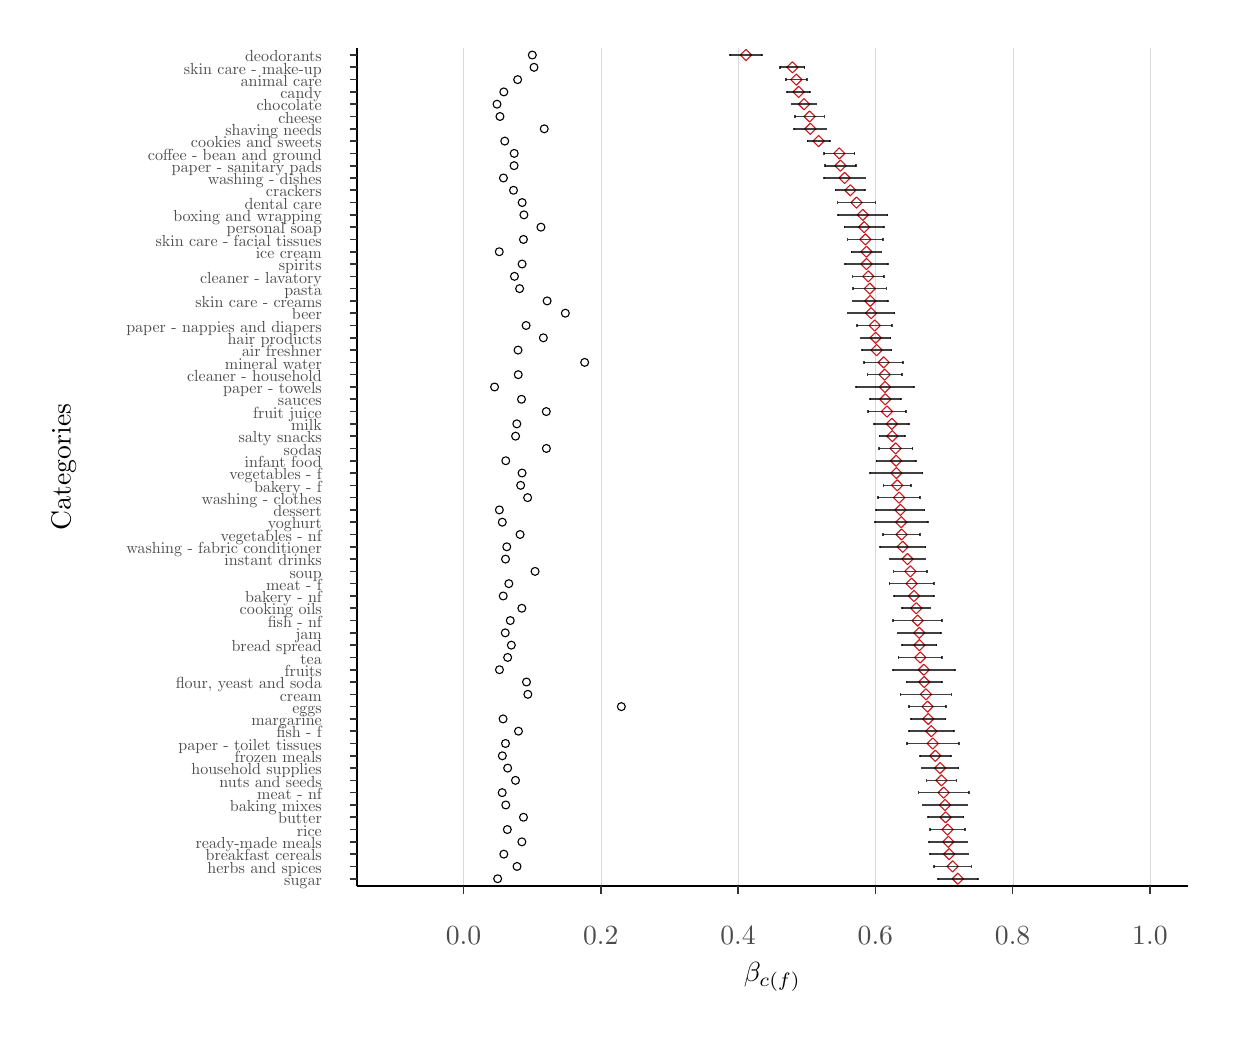
\begin{tikzpicture}[x=1pt,y=1pt]
\definecolor{fillColor}{RGB}{255,255,255}
\path[use as bounding box,fill=fillColor,fill opacity=0.00] (0,0) rectangle (433.62,361.35);
\begin{scope}
\path[clip] (  0.00,  0.00) rectangle (433.62,361.35);
\definecolor{drawColor}{RGB}{255,255,255}
\definecolor{fillColor}{RGB}{255,255,255}

\path[draw=drawColor,line width= 0.6pt,line join=round,line cap=round,fill=fillColor] (  0.00,  0.00) rectangle (433.62,361.35);
\end{scope}
\begin{scope}
\path[clip] (119.04, 51.15) rectangle (419.17,354.12);
\definecolor{drawColor}{RGB}{255,255,255}

\path[draw=drawColor,line width= 0.3pt,line join=round] (132.68, 51.15) --
	(132.68,354.12);

\path[draw=drawColor,line width= 0.3pt,line join=round] (182.29, 51.15) --
	(182.29,354.12);

\path[draw=drawColor,line width= 0.3pt,line join=round] (231.90, 51.15) --
	(231.90,354.12);

\path[draw=drawColor,line width= 0.3pt,line join=round] (281.51, 51.15) --
	(281.51,354.12);

\path[draw=drawColor,line width= 0.3pt,line join=round] (331.11, 51.15) --
	(331.11,354.12);

\path[draw=drawColor,line width= 0.3pt,line join=round] (380.72, 51.15) --
	(380.72,354.12);
\definecolor{drawColor}{gray}{0.85}

\path[draw=drawColor,line width= 0.1pt,line join=round] (157.49, 51.15) --
	(157.49,354.12);

\path[draw=drawColor,line width= 0.1pt,line join=round] (207.09, 51.15) --
	(207.09,354.12);

\path[draw=drawColor,line width= 0.1pt,line join=round] (256.70, 51.15) --
	(256.70,354.12);

\path[draw=drawColor,line width= 0.1pt,line join=round] (306.31, 51.15) --
	(306.31,354.12);

\path[draw=drawColor,line width= 0.1pt,line join=round] (355.92, 51.15) --
	(355.92,354.12);

\path[draw=drawColor,line width= 0.1pt,line join=round] (405.52, 51.15) --
	(405.52,354.12);
\definecolor{drawColor}{RGB}{0,0,0}

\path[draw=drawColor,line width= 0.4pt,line join=round,line cap=round] (177.19,244.84) circle (  1.43);

\path[draw=drawColor,line width= 0.4pt,line join=round,line cap=round] (177.05,342.57) circle (  1.43);

\path[draw=drawColor,line width= 0.4pt,line join=round,line cap=round] (178.14,195.97) circle (  1.43);

\path[draw=drawColor,line width= 0.4pt,line join=round,line cap=round] (171.83,155.99) circle (  1.43);

\path[draw=drawColor,line width= 0.4pt,line join=round,line cap=round] (172.76, 80.47) circle (  1.43);

\path[draw=drawColor,line width= 0.4pt,line join=round,line cap=round] (194.28,258.17) circle (  1.43);

\path[draw=drawColor,line width= 0.4pt,line join=round,line cap=round] (179.32,293.71) circle (  1.43);

\path[draw=drawColor,line width= 0.4pt,line join=round,line cap=round] (174.77,138.22) circle (  1.43);

\path[draw=drawColor,line width= 0.4pt,line join=round,line cap=round] (172.06, 62.70) circle (  1.43);

\path[draw=drawColor,line width= 0.4pt,line join=round,line cap=round] (179.16, 76.03) circle (  1.43);

\path[draw=drawColor,line width= 0.4pt,line join=round,line cap=round] (172.05,338.13) circle (  1.43);

\path[draw=drawColor,line width= 0.4pt,line join=round,line cap=round] (170.66,329.25) circle (  1.43);

\path[draw=drawColor,line width= 0.4pt,line join=round,line cap=round] (169.59,333.69) circle (  1.43);

\path[draw=drawColor,line width= 0.4pt,line join=round,line cap=round] (177.26,235.96) circle (  1.43);

\path[draw=drawColor,line width= 0.4pt,line join=round,line cap=round] (175.90,271.49) circle (  1.43);

\path[draw=drawColor,line width= 0.4pt,line join=round,line cap=round] (175.80,315.92) circle (  1.43);

\path[draw=drawColor,line width= 0.4pt,line join=round,line cap=round] (172.39,320.36) circle (  1.43);

\path[draw=drawColor,line width= 0.4pt,line join=round,line cap=round] (178.56,151.55) circle (  1.43);

\path[draw=drawColor,line width= 0.4pt,line join=round,line cap=round] (175.55,302.59) circle (  1.43);

\path[draw=drawColor,line width= 0.4pt,line join=round,line cap=round] (180.74,120.45) circle (  1.43);

\path[draw=drawColor,line width= 0.4pt,line join=round,line cap=round] (178.68,298.15) circle (  1.43);

\path[draw=drawColor,line width= 0.4pt,line join=round,line cap=round] (182.35,351.46) circle (  1.43);

\path[draw=drawColor,line width= 0.4pt,line join=round,line cap=round] (170.44,187.09) circle (  1.43);

\path[draw=drawColor,line width= 0.4pt,line join=round,line cap=round] (214.52,116.01) circle (  1.43);

\path[draw=drawColor,line width= 0.4pt,line join=round,line cap=round] (177.35,107.13) circle (  1.43);

\path[draw=drawColor,line width= 0.4pt,line join=round,line cap=round] (174.38,147.11) circle (  1.43);

\path[draw=drawColor,line width= 0.4pt,line join=round,line cap=round] (180.24,124.90) circle (  1.43);

\path[draw=drawColor,line width= 0.4pt,line join=round,line cap=round] (171.52, 98.24) circle (  1.43);

\path[draw=drawColor,line width= 0.4pt,line join=round,line cap=round] (187.40,222.63) circle (  1.43);

\path[draw=drawColor,line width= 0.4pt,line join=round,line cap=round] (170.48,129.34) circle (  1.43);

\path[draw=drawColor,line width= 0.4pt,line join=round,line cap=round] (186.34,249.28) circle (  1.43);

\path[draw=drawColor,line width= 0.4pt,line join=round,line cap=round] (176.82, 58.26) circle (  1.43);

\path[draw=drawColor,line width= 0.4pt,line join=round,line cap=round] (173.44, 93.80) circle (  1.43);

\path[draw=drawColor,line width= 0.4pt,line join=round,line cap=round] (170.41,280.38) circle (  1.43);

\path[draw=drawColor,line width= 0.4pt,line join=round,line cap=round] (172.76,204.86) circle (  1.43);

\path[draw=drawColor,line width= 0.4pt,line join=round,line cap=round] (172.67,169.32) circle (  1.43);

\path[draw=drawColor,line width= 0.4pt,line join=round,line cap=round] (172.57,142.67) circle (  1.43);

\path[draw=drawColor,line width= 0.4pt,line join=round,line cap=round] (171.78,111.57) circle (  1.43);

\path[draw=drawColor,line width= 0.4pt,line join=round,line cap=round] (173.87,160.44) circle (  1.43);

\path[draw=drawColor,line width= 0.4pt,line join=round,line cap=round] (171.46, 84.92) circle (  1.43);

\path[draw=drawColor,line width= 0.4pt,line join=round,line cap=round] (176.75,218.19) circle (  1.43);

\path[draw=drawColor,line width= 0.4pt,line join=round,line cap=round] (201.27,240.40) circle (  1.43);

\path[draw=drawColor,line width= 0.4pt,line join=round,line cap=round] (176.27, 89.36) circle (  1.43);

\path[draw=drawColor,line width= 0.4pt,line join=round,line cap=round] (180.10,253.73) circle (  1.43);

\path[draw=drawColor,line width= 0.4pt,line join=round,line cap=round] (175.76,311.48) circle (  1.43);

\path[draw=drawColor,line width= 0.4pt,line join=round,line cap=round] (172.66,102.69) circle (  1.43);

\path[draw=drawColor,line width= 0.4pt,line join=round,line cap=round] (168.71,231.51) circle (  1.43);

\path[draw=drawColor,line width= 0.4pt,line join=round,line cap=round] (177.76,267.05) circle (  1.43);

\path[draw=drawColor,line width= 0.4pt,line join=round,line cap=round] (185.47,289.26) circle (  1.43);

\path[draw=drawColor,line width= 0.4pt,line join=round,line cap=round] (178.58, 67.15) circle (  1.43);

\path[draw=drawColor,line width= 0.4pt,line join=round,line cap=round] (173.32, 71.59) circle (  1.43);

\path[draw=drawColor,line width= 0.4pt,line join=round,line cap=round] (176.30,213.74) circle (  1.43);

\path[draw=drawColor,line width= 0.4pt,line join=round,line cap=round] (178.44,227.07) circle (  1.43);

\path[draw=drawColor,line width= 0.4pt,line join=round,line cap=round] (186.66,324.80) circle (  1.43);

\path[draw=drawColor,line width= 0.4pt,line join=round,line cap=round] (187.70,262.61) circle (  1.43);

\path[draw=drawColor,line width= 0.4pt,line join=round,line cap=round] (179.15,284.82) circle (  1.43);

\path[draw=drawColor,line width= 0.4pt,line join=round,line cap=round] (182.96,347.02) circle (  1.43);

\path[draw=drawColor,line width= 0.4pt,line join=round,line cap=round] (187.44,209.30) circle (  1.43);

\path[draw=drawColor,line width= 0.4pt,line join=round,line cap=round] (183.34,164.88) circle (  1.43);

\path[draw=drawColor,line width= 0.4pt,line join=round,line cap=round] (178.66,275.94) circle (  1.43);

\path[draw=drawColor,line width= 0.4pt,line join=round,line cap=round] (169.83, 53.82) circle (  1.43);

\path[draw=drawColor,line width= 0.4pt,line join=round,line cap=round] (173.44,133.78) circle (  1.43);

\path[draw=drawColor,line width= 0.4pt,line join=round,line cap=round] (178.64,200.42) circle (  1.43);

\path[draw=drawColor,line width= 0.4pt,line join=round,line cap=round] (177.93,178.21) circle (  1.43);

\path[draw=drawColor,line width= 0.4pt,line join=round,line cap=round] (180.66,191.53) circle (  1.43);

\path[draw=drawColor,line width= 0.4pt,line join=round,line cap=round] (171.91,307.03) circle (  1.43);

\path[draw=drawColor,line width= 0.4pt,line join=round,line cap=round] (173.12,173.76) circle (  1.43);

\path[draw=drawColor,line width= 0.4pt,line join=round,line cap=round] (171.50,182.65) circle (  1.43);
\definecolor{drawColor}{RGB}{203,24,29}

\path[draw=drawColor,line width= 0.4pt,line join=round,line cap=round] (304.74,244.84) --
	(306.76,246.86) --
	(308.78,244.84) --
	(306.76,242.82) --
	cycle;

\path[draw=drawColor,line width= 0.4pt,line join=round,line cap=round] (275.72,342.57) --
	(277.74,344.59) --
	(279.76,342.57) --
	(277.74,340.56) --
	cycle;

\path[draw=drawColor,line width= 0.4pt,line join=round,line cap=round] (312.19,195.97) --
	(314.21,197.99) --
	(316.22,195.97) --
	(314.21,193.96) --
	cycle;

\path[draw=drawColor,line width= 0.4pt,line join=round,line cap=round] (318.25,155.99) --
	(320.27,158.01) --
	(322.29,155.99) --
	(320.27,153.98) --
	cycle;

\path[draw=drawColor,line width= 0.4pt,line join=round,line cap=round] (329.46, 80.47) --
	(331.47, 82.49) --
	(333.49, 80.47) --
	(331.47, 78.46) --
	cycle;

\path[draw=drawColor,line width= 0.4pt,line join=round,line cap=round] (302.74,258.17) --
	(304.76,260.19) --
	(306.78,258.17) --
	(304.76,256.15) --
	cycle;

\path[draw=drawColor,line width= 0.4pt,line join=round,line cap=round] (299.76,293.71) --
	(301.77,295.72) --
	(303.79,293.71) --
	(301.77,291.69) --
	cycle;

\path[draw=drawColor,line width= 0.4pt,line join=round,line cap=round] (320.21,138.22) --
	(322.22,140.24) --
	(324.24,138.22) --
	(322.22,136.21) --
	cycle;

\path[draw=drawColor,line width= 0.4pt,line join=round,line cap=round] (330.97, 62.70) --
	(332.99, 64.72) --
	(335.01, 62.70) --
	(332.99, 60.69) --
	cycle;

\path[draw=drawColor,line width= 0.4pt,line join=round,line cap=round] (329.68, 76.03) --
	(331.70, 78.05) --
	(333.72, 76.03) --
	(331.70, 74.01) --
	cycle;

\path[draw=drawColor,line width= 0.4pt,line join=round,line cap=round] (276.58,338.13) --
	(278.59,340.15) --
	(280.61,338.13) --
	(278.59,336.11) --
	cycle;

\path[draw=drawColor,line width= 0.4pt,line join=round,line cap=round] (280.52,329.25) --
	(282.53,331.26) --
	(284.55,329.25) --
	(282.53,327.23) --
	cycle;

\path[draw=drawColor,line width= 0.4pt,line join=round,line cap=round] (278.52,333.69) --
	(280.54,335.71) --
	(282.56,333.69) --
	(280.54,331.67) --
	cycle;

\path[draw=drawColor,line width= 0.4pt,line join=round,line cap=round] (307.64,235.96) --
	(309.66,237.97) --
	(311.67,235.96) --
	(309.66,233.94) --
	cycle;

\path[draw=drawColor,line width= 0.4pt,line join=round,line cap=round] (301.74,271.49) --
	(303.75,273.51) --
	(305.77,271.49) --
	(303.75,269.48) --
	cycle;

\path[draw=drawColor,line width= 0.4pt,line join=round,line cap=round] (291.25,315.92) --
	(293.26,317.94) --
	(295.28,315.92) --
	(293.26,313.90) --
	cycle;

\path[draw=drawColor,line width= 0.4pt,line join=round,line cap=round] (283.76,320.36) --
	(285.78,322.38) --
	(287.80,320.36) --
	(285.78,318.34) --
	cycle;

\path[draw=drawColor,line width= 0.4pt,line join=round,line cap=round] (319.07,151.55) --
	(321.09,153.57) --
	(323.11,151.55) --
	(321.09,149.53) --
	cycle;

\path[draw=drawColor,line width= 0.4pt,line join=round,line cap=round] (295.25,302.59) --
	(297.27,304.61) --
	(299.28,302.59) --
	(297.27,300.57) --
	cycle;

\path[draw=drawColor,line width= 0.4pt,line join=round,line cap=round] (322.57,120.45) --
	(324.59,122.47) --
	(326.61,120.45) --
	(324.59,118.44) --
	cycle;

\path[draw=drawColor,line width= 0.4pt,line join=round,line cap=round] (297.48,298.15) --
	(299.50,300.17) --
	(301.52,298.15) --
	(299.50,296.13) --
	cycle;

\path[draw=drawColor,line width= 0.4pt,line join=round,line cap=round] (257.54,351.46) --
	(259.56,353.48) --
	(261.57,351.46) --
	(259.56,349.44) --
	cycle;

\path[draw=drawColor,line width= 0.4pt,line join=round,line cap=round] (313.35,187.09) --
	(315.37,189.11) --
	(317.39,187.09) --
	(315.37,185.07) --
	cycle;

\path[draw=drawColor,line width= 0.4pt,line join=round,line cap=round] (323.14,116.01) --
	(325.15,118.03) --
	(327.17,116.01) --
	(325.15,113.99) --
	cycle;

\path[draw=drawColor,line width= 0.4pt,line join=round,line cap=round] (324.50,107.13) --
	(326.52,109.14) --
	(328.53,107.13) --
	(326.52,105.11) --
	cycle;

\path[draw=drawColor,line width= 0.4pt,line join=round,line cap=round] (319.57,147.11) --
	(321.58,149.13) --
	(323.60,147.11) --
	(321.58,145.09) --
	cycle;

\path[draw=drawColor,line width= 0.4pt,line join=round,line cap=round] (321.93,124.90) --
	(323.95,126.91) --
	(325.97,124.90) --
	(323.95,122.88) --
	cycle;

\path[draw=drawColor,line width= 0.4pt,line join=round,line cap=round] (325.95, 98.24) --
	(327.97,100.26) --
	(329.99, 98.24) --
	(327.97, 96.23) --
	cycle;

\path[draw=drawColor,line width= 0.4pt,line join=round,line cap=round] (308.49,222.63) --
	(310.51,224.65) --
	(312.52,222.63) --
	(310.51,220.61) --
	cycle;

\path[draw=drawColor,line width= 0.4pt,line join=round,line cap=round] (321.80,129.34) --
	(323.82,131.36) --
	(325.84,129.34) --
	(323.82,127.32) --
	cycle;

\path[draw=drawColor,line width= 0.4pt,line join=round,line cap=round] (304.38,249.28) --
	(306.40,251.30) --
	(308.42,249.28) --
	(306.40,247.27) --
	cycle;

\path[draw=drawColor,line width= 0.4pt,line join=round,line cap=round] (332.22, 58.26) --
	(334.24, 60.28) --
	(336.25, 58.26) --
	(334.24, 56.24) --
	cycle;

\path[draw=drawColor,line width= 0.4pt,line join=round,line cap=round] (327.68, 93.80) --
	(329.69, 95.82) --
	(331.71, 93.80) --
	(329.69, 91.78) --
	cycle;

\path[draw=drawColor,line width= 0.4pt,line join=round,line cap=round] (301.07,280.38) --
	(303.08,282.40) --
	(305.10,280.38) --
	(303.08,278.36) --
	cycle;

\path[draw=drawColor,line width= 0.4pt,line join=round,line cap=round] (311.78,204.86) --
	(313.80,206.88) --
	(315.81,204.86) --
	(313.80,202.84) --
	cycle;

\path[draw=drawColor,line width= 0.4pt,line join=round,line cap=round] (315.91,169.32) --
	(317.93,171.34) --
	(319.95,169.32) --
	(317.93,167.30) --
	cycle;

\path[draw=drawColor,line width= 0.4pt,line join=round,line cap=round] (320.16,142.67) --
	(322.17,144.68) --
	(324.19,142.67) --
	(322.17,140.65) --
	cycle;

\path[draw=drawColor,line width= 0.4pt,line join=round,line cap=round] (323.40,111.57) --
	(325.42,113.59) --
	(327.44,111.57) --
	(325.42,109.55) --
	cycle;

\path[draw=drawColor,line width= 0.4pt,line join=round,line cap=round] (317.37,160.44) --
	(319.39,162.45) --
	(321.41,160.44) --
	(319.39,158.42) --
	cycle;

\path[draw=drawColor,line width= 0.4pt,line join=round,line cap=round] (328.97, 84.92) --
	(330.99, 86.93) --
	(333.01, 84.92) --
	(330.99, 82.90) --
	cycle;

\path[draw=drawColor,line width= 0.4pt,line join=round,line cap=round] (310.23,218.19) --
	(312.25,220.20) --
	(314.27,218.19) --
	(312.25,216.17) --
	cycle;

\path[draw=drawColor,line width= 0.4pt,line join=round,line cap=round] (307.31,240.40) --
	(309.33,242.42) --
	(311.35,240.40) --
	(309.33,238.38) --
	cycle;

\path[draw=drawColor,line width= 0.4pt,line join=round,line cap=round] (328.18, 89.36) --
	(330.19, 91.38) --
	(332.21, 89.36) --
	(330.19, 87.34) --
	cycle;

\path[draw=drawColor,line width= 0.4pt,line join=round,line cap=round] (304.06,253.73) --
	(306.08,255.74) --
	(308.10,253.73) --
	(306.08,251.71) --
	cycle;

\path[draw=drawColor,line width= 0.4pt,line join=round,line cap=round] (291.65,311.48) --
	(293.67,313.49) --
	(295.69,311.48) --
	(293.67,309.46) --
	cycle;

\path[draw=drawColor,line width= 0.4pt,line join=round,line cap=round] (325.01,102.69) --
	(327.03,104.70) --
	(329.05,102.69) --
	(327.03,100.67) --
	cycle;

\path[draw=drawColor,line width= 0.4pt,line join=round,line cap=round] (307.76,231.51) --
	(309.78,233.53) --
	(311.80,231.51) --
	(309.78,229.50) --
	cycle;

\path[draw=drawColor,line width= 0.4pt,line join=round,line cap=round] (302.29,267.05) --
	(304.30,269.07) --
	(306.32,267.05) --
	(304.30,265.04) --
	cycle;

\path[draw=drawColor,line width= 0.4pt,line join=round,line cap=round] (300.25,289.26) --
	(302.27,291.28) --
	(304.29,289.26) --
	(302.27,287.25) --
	cycle;

\path[draw=drawColor,line width= 0.4pt,line join=round,line cap=round] (330.65, 67.15) --
	(332.67, 69.16) --
	(334.69, 67.15) --
	(332.67, 65.13) --
	cycle;

\path[draw=drawColor,line width= 0.4pt,line join=round,line cap=round] (330.38, 71.59) --
	(332.39, 73.61) --
	(334.41, 71.59) --
	(332.39, 69.57) --
	cycle;

\path[draw=drawColor,line width= 0.4pt,line join=round,line cap=round] (310.40,213.74) --
	(312.42,215.76) --
	(314.44,213.74) --
	(312.42,211.73) --
	cycle;

\path[draw=drawColor,line width= 0.4pt,line join=round,line cap=round] (307.88,227.07) --
	(309.90,229.09) --
	(311.91,227.07) --
	(309.90,225.05) --
	cycle;

\path[draw=drawColor,line width= 0.4pt,line join=round,line cap=round] (280.77,324.80) --
	(282.79,326.82) --
	(284.81,324.80) --
	(282.79,322.79) --
	cycle;

\path[draw=drawColor,line width= 0.4pt,line join=round,line cap=round] (302.45,262.61) --
	(304.47,264.63) --
	(306.48,262.61) --
	(304.47,260.59) --
	cycle;

\path[draw=drawColor,line width= 0.4pt,line join=round,line cap=round] (300.68,284.82) --
	(302.70,286.84) --
	(304.72,284.82) --
	(302.70,282.80) --
	cycle;

\path[draw=drawColor,line width= 0.4pt,line join=round,line cap=round] (274.33,347.02) --
	(276.35,349.03) --
	(278.36,347.02) --
	(276.35,345.00) --
	cycle;

\path[draw=drawColor,line width= 0.4pt,line join=round,line cap=round] (311.62,209.30) --
	(313.64,211.32) --
	(315.65,209.30) --
	(313.64,207.28) --
	cycle;

\path[draw=drawColor,line width= 0.4pt,line join=round,line cap=round] (316.95,164.88) --
	(318.97,166.90) --
	(320.98,164.88) --
	(318.97,162.86) --
	cycle;

\path[draw=drawColor,line width= 0.4pt,line join=round,line cap=round] (301.11,275.94) --
	(303.13,277.95) --
	(305.15,275.94) --
	(303.13,273.92) --
	cycle;

\path[draw=drawColor,line width= 0.4pt,line join=round,line cap=round] (334.09, 53.82) --
	(336.11, 55.84) --
	(338.13, 53.82) --
	(336.11, 51.80) --
	cycle;

\path[draw=drawColor,line width= 0.4pt,line join=round,line cap=round] (320.50,133.78) --
	(322.51,135.80) --
	(324.53,133.78) --
	(322.51,131.76) --
	cycle;

\path[draw=drawColor,line width= 0.4pt,line join=round,line cap=round] (311.89,200.42) --
	(313.91,202.43) --
	(315.92,200.42) --
	(313.91,198.40) --
	cycle;

\path[draw=drawColor,line width= 0.4pt,line join=round,line cap=round] (313.76,178.21) --
	(315.77,180.22) --
	(317.79,178.21) --
	(315.77,176.19) --
	cycle;

\path[draw=drawColor,line width= 0.4pt,line join=round,line cap=round] (312.87,191.53) --
	(314.89,193.55) --
	(316.91,191.53) --
	(314.89,189.51) --
	cycle;

\path[draw=drawColor,line width= 0.4pt,line join=round,line cap=round] (293.18,307.03) --
	(295.20,309.05) --
	(297.22,307.03) --
	(295.20,305.02) --
	cycle;

\path[draw=drawColor,line width= 0.4pt,line join=round,line cap=round] (314.17,173.76) --
	(316.19,175.78) --
	(318.21,173.76) --
	(316.19,171.75) --
	cycle;

\path[draw=drawColor,line width= 0.4pt,line join=round,line cap=round] (313.62,182.65) --
	(315.64,184.67) --
	(317.66,182.65) --
	(315.64,180.63) --
	cycle;
\definecolor{drawColor}{RGB}{0,0,0}

\path[draw=drawColor,draw opacity=0.75,line width= 0.6pt,line join=round] (312.14,244.40) --
	(312.14,245.29);

\path[draw=drawColor,draw opacity=0.75,line width= 0.6pt,line join=round] (312.14,244.84) --
	(301.37,244.84);

\path[draw=drawColor,draw opacity=0.75,line width= 0.6pt,line join=round] (301.37,244.40) --
	(301.37,245.29);

\path[draw=drawColor,draw opacity=0.75,line width= 0.6pt,line join=round] (281.58,342.13) --
	(281.58,343.02);

\path[draw=drawColor,draw opacity=0.75,line width= 0.6pt,line join=round] (281.58,342.57) --
	(273.90,342.57);

\path[draw=drawColor,draw opacity=0.75,line width= 0.6pt,line join=round] (273.90,342.13) --
	(273.90,343.02);

\path[draw=drawColor,draw opacity=0.75,line width= 0.6pt,line join=round] (319.15,195.53) --
	(319.15,196.42);

\path[draw=drawColor,draw opacity=0.75,line width= 0.6pt,line join=round] (319.15,195.97) --
	(309.26,195.97);

\path[draw=drawColor,draw opacity=0.75,line width= 0.6pt,line join=round] (309.26,195.53) --
	(309.26,196.42);

\path[draw=drawColor,draw opacity=0.75,line width= 0.6pt,line join=round] (327.51,155.55) --
	(327.51,156.44);

\path[draw=drawColor,draw opacity=0.75,line width= 0.6pt,line join=round] (327.51,155.99) --
	(313.03,155.99);

\path[draw=drawColor,draw opacity=0.75,line width= 0.6pt,line join=round] (313.03,155.55) --
	(313.03,156.44);

\path[draw=drawColor,draw opacity=0.75,line width= 0.6pt,line join=round] (339.57, 80.03) --
	(339.57, 80.92);

\path[draw=drawColor,draw opacity=0.75,line width= 0.6pt,line join=round] (339.57, 80.47) --
	(323.38, 80.47);

\path[draw=drawColor,draw opacity=0.75,line width= 0.6pt,line join=round] (323.38, 80.03) --
	(323.38, 80.92);

\path[draw=drawColor,draw opacity=0.75,line width= 0.6pt,line join=round] (313.25,257.72) --
	(313.25,258.61);

\path[draw=drawColor,draw opacity=0.75,line width= 0.6pt,line join=round] (313.25,258.17) --
	(296.27,258.17);

\path[draw=drawColor,draw opacity=0.75,line width= 0.6pt,line join=round] (296.27,257.72) --
	(296.27,258.61);

\path[draw=drawColor,draw opacity=0.75,line width= 0.6pt,line join=round] (310.71,293.26) --
	(310.71,294.15);

\path[draw=drawColor,draw opacity=0.75,line width= 0.6pt,line join=round] (310.71,293.71) --
	(292.84,293.71);

\path[draw=drawColor,draw opacity=0.75,line width= 0.6pt,line join=round] (292.84,293.26) --
	(292.84,294.15);

\path[draw=drawColor,draw opacity=0.75,line width= 0.6pt,line join=round] (328.42,137.78) --
	(328.42,138.67);

\path[draw=drawColor,draw opacity=0.75,line width= 0.6pt,line join=round] (328.42,138.22) --
	(316.03,138.22);

\path[draw=drawColor,draw opacity=0.75,line width= 0.6pt,line join=round] (316.03,137.78) --
	(316.03,138.67);

\path[draw=drawColor,draw opacity=0.75,line width= 0.6pt,line join=round] (339.92, 62.26) --
	(339.92, 63.15);

\path[draw=drawColor,draw opacity=0.75,line width= 0.6pt,line join=round] (339.92, 62.70) --
	(326.06, 62.70);

\path[draw=drawColor,draw opacity=0.75,line width= 0.6pt,line join=round] (326.06, 62.26) --
	(326.06, 63.15);

\path[draw=drawColor,draw opacity=0.75,line width= 0.6pt,line join=round] (338.16, 75.59) --
	(338.16, 76.48);

\path[draw=drawColor,draw opacity=0.75,line width= 0.6pt,line join=round] (338.16, 76.03) --
	(325.24, 76.03);

\path[draw=drawColor,draw opacity=0.75,line width= 0.6pt,line join=round] (325.24, 75.59) --
	(325.24, 76.48);

\path[draw=drawColor,draw opacity=0.75,line width= 0.6pt,line join=round] (282.75,337.69) --
	(282.75,338.57);

\path[draw=drawColor,draw opacity=0.75,line width= 0.6pt,line join=round] (282.75,338.13) --
	(274.44,338.13);

\path[draw=drawColor,draw opacity=0.75,line width= 0.6pt,line join=round] (274.44,337.69) --
	(274.44,338.57);

\path[draw=drawColor,draw opacity=0.75,line width= 0.6pt,line join=round] (287.88,328.80) --
	(287.88,329.69);

\path[draw=drawColor,draw opacity=0.75,line width= 0.6pt,line join=round] (287.88,329.25) --
	(277.19,329.25);

\path[draw=drawColor,draw opacity=0.75,line width= 0.6pt,line join=round] (277.19,328.80) --
	(277.19,329.69);

\path[draw=drawColor,draw opacity=0.75,line width= 0.6pt,line join=round] (285.02,333.24) --
	(285.02,334.13);

\path[draw=drawColor,draw opacity=0.75,line width= 0.6pt,line join=round] (285.02,333.69) --
	(276.06,333.69);

\path[draw=drawColor,draw opacity=0.75,line width= 0.6pt,line join=round] (276.06,333.24) --
	(276.06,334.13);

\path[draw=drawColor,draw opacity=0.75,line width= 0.6pt,line join=round] (315.85,235.51) --
	(315.85,236.40);

\path[draw=drawColor,draw opacity=0.75,line width= 0.6pt,line join=round] (315.85,235.96) --
	(303.47,235.96);

\path[draw=drawColor,draw opacity=0.75,line width= 0.6pt,line join=round] (303.47,235.51) --
	(303.47,236.40);

\path[draw=drawColor,draw opacity=0.75,line width= 0.6pt,line join=round] (309.41,271.05) --
	(309.41,271.94);

\path[draw=drawColor,draw opacity=0.75,line width= 0.6pt,line join=round] (309.41,271.49) --
	(298.10,271.49);

\path[draw=drawColor,draw opacity=0.75,line width= 0.6pt,line join=round] (298.10,271.05) --
	(298.10,271.94);

\path[draw=drawColor,draw opacity=0.75,line width= 0.6pt,line join=round] (298.80,315.47) --
	(298.80,316.36);

\path[draw=drawColor,draw opacity=0.75,line width= 0.6pt,line join=round] (298.80,315.92) --
	(287.73,315.92);

\path[draw=drawColor,draw opacity=0.75,line width= 0.6pt,line join=round] (287.73,315.47) --
	(287.73,316.36);

\path[draw=drawColor,draw opacity=0.75,line width= 0.6pt,line join=round] (289.82,319.92) --
	(289.82,320.81);

\path[draw=drawColor,draw opacity=0.75,line width= 0.6pt,line join=round] (289.82,320.36) --
	(281.74,320.36);

\path[draw=drawColor,draw opacity=0.75,line width= 0.6pt,line join=round] (281.74,319.92) --
	(281.74,320.81);

\path[draw=drawColor,draw opacity=0.75,line width= 0.6pt,line join=round] (326.21,151.11) --
	(326.21,152.00);

\path[draw=drawColor,draw opacity=0.75,line width= 0.6pt,line join=round] (326.21,151.55) --
	(315.98,151.55);

\path[draw=drawColor,draw opacity=0.75,line width= 0.6pt,line join=round] (315.98,151.11) --
	(315.98,152.00);

\path[draw=drawColor,draw opacity=0.75,line width= 0.6pt,line join=round] (302.64,302.15) --
	(302.64,303.04);

\path[draw=drawColor,draw opacity=0.75,line width= 0.6pt,line join=round] (302.64,302.59) --
	(291.90,302.59);

\path[draw=drawColor,draw opacity=0.75,line width= 0.6pt,line join=round] (291.90,302.15) --
	(291.90,303.04);

\path[draw=drawColor,draw opacity=0.75,line width= 0.6pt,line join=round] (333.81,120.01) --
	(333.81,120.90);

\path[draw=drawColor,draw opacity=0.75,line width= 0.6pt,line join=round] (333.81,120.45) --
	(315.37,120.45);

\path[draw=drawColor,draw opacity=0.75,line width= 0.6pt,line join=round] (315.37,120.01) --
	(315.37,120.90);

\path[draw=drawColor,draw opacity=0.75,line width= 0.6pt,line join=round] (306.32,297.70) --
	(306.32,298.59);

\path[draw=drawColor,draw opacity=0.75,line width= 0.6pt,line join=round] (306.32,298.15) --
	(292.68,298.15);

\path[draw=drawColor,draw opacity=0.75,line width= 0.6pt,line join=round] (292.68,297.70) --
	(292.68,298.59);

\path[draw=drawColor,draw opacity=0.75,line width= 0.6pt,line join=round] (265.41,351.01) --
	(265.41,351.90);

\path[draw=drawColor,draw opacity=0.75,line width= 0.6pt,line join=round] (265.41,351.46) --
	(253.70,351.46);

\path[draw=drawColor,draw opacity=0.75,line width= 0.6pt,line join=round] (253.70,351.01) --
	(253.70,351.90);

\path[draw=drawColor,draw opacity=0.75,line width= 0.6pt,line join=round] (324.11,186.65) --
	(324.11,187.53);

\path[draw=drawColor,draw opacity=0.75,line width= 0.6pt,line join=round] (324.11,187.09) --
	(306.62,187.09);

\path[draw=drawColor,draw opacity=0.75,line width= 0.6pt,line join=round] (306.62,186.65) --
	(306.62,187.53);

\path[draw=drawColor,draw opacity=0.75,line width= 0.6pt,line join=round] (331.85,115.57) --
	(331.85,116.46);

\path[draw=drawColor,draw opacity=0.75,line width= 0.6pt,line join=round] (331.85,116.01) --
	(318.45,116.01);

\path[draw=drawColor,draw opacity=0.75,line width= 0.6pt,line join=round] (318.45,115.57) --
	(318.45,116.46);

\path[draw=drawColor,draw opacity=0.75,line width= 0.6pt,line join=round] (334.63,106.68) --
	(334.63,107.57);

\path[draw=drawColor,draw opacity=0.75,line width= 0.6pt,line join=round] (334.63,107.13) --
	(318.40,107.13);

\path[draw=drawColor,draw opacity=0.75,line width= 0.6pt,line join=round] (318.40,106.68) --
	(318.40,107.57);

\path[draw=drawColor,draw opacity=0.75,line width= 0.6pt,line join=round] (330.39,146.66) --
	(330.39,147.55);

\path[draw=drawColor,draw opacity=0.75,line width= 0.6pt,line join=round] (330.39,147.11) --
	(312.77,147.11);

\path[draw=drawColor,draw opacity=0.75,line width= 0.6pt,line join=round] (312.77,146.66) --
	(312.77,147.55);

\path[draw=drawColor,draw opacity=0.75,line width= 0.6pt,line join=round] (330.39,124.45) --
	(330.39,125.34);

\path[draw=drawColor,draw opacity=0.75,line width= 0.6pt,line join=round] (330.39,124.90) --
	(317.51,124.90);

\path[draw=drawColor,draw opacity=0.75,line width= 0.6pt,line join=round] (317.51,124.45) --
	(317.51,125.34);

\path[draw=drawColor,draw opacity=0.75,line width= 0.6pt,line join=round] (333.57, 97.80) --
	(333.57, 98.69);

\path[draw=drawColor,draw opacity=0.75,line width= 0.6pt,line join=round] (333.57, 98.24) --
	(322.38, 98.24);

\path[draw=drawColor,draw opacity=0.75,line width= 0.6pt,line join=round] (322.38, 97.80) --
	(322.38, 98.69);

\path[draw=drawColor,draw opacity=0.75,line width= 0.6pt,line join=round] (317.39,222.18) --
	(317.39,223.07);

\path[draw=drawColor,draw opacity=0.75,line width= 0.6pt,line join=round] (317.39,222.63) --
	(303.63,222.63);

\path[draw=drawColor,draw opacity=0.75,line width= 0.6pt,line join=round] (303.63,222.18) --
	(303.63,223.07);

\path[draw=drawColor,draw opacity=0.75,line width= 0.6pt,line join=round] (335.04,128.90) --
	(335.04,129.78);

\path[draw=drawColor,draw opacity=0.75,line width= 0.6pt,line join=round] (335.04,129.34) --
	(312.60,129.34);

\path[draw=drawColor,draw opacity=0.75,line width= 0.6pt,line join=round] (312.60,128.90) --
	(312.60,129.78);

\path[draw=drawColor,draw opacity=0.75,line width= 0.6pt,line join=round] (311.82,248.84) --
	(311.82,249.73);

\path[draw=drawColor,draw opacity=0.75,line width= 0.6pt,line join=round] (311.82,249.28) --
	(300.98,249.28);

\path[draw=drawColor,draw opacity=0.75,line width= 0.6pt,line join=round] (300.98,248.84) --
	(300.98,249.73);

\path[draw=drawColor,draw opacity=0.75,line width= 0.6pt,line join=round] (340.99, 57.82) --
	(340.99, 58.71);

\path[draw=drawColor,draw opacity=0.75,line width= 0.6pt,line join=round] (340.99, 58.26) --
	(327.48, 58.26);

\path[draw=drawColor,draw opacity=0.75,line width= 0.6pt,line join=round] (327.48, 57.82) --
	(327.48, 58.71);

\path[draw=drawColor,draw opacity=0.75,line width= 0.6pt,line join=round] (336.38, 93.36) --
	(336.38, 94.24);

\path[draw=drawColor,draw opacity=0.75,line width= 0.6pt,line join=round] (336.38, 93.80) --
	(323.01, 93.80);

\path[draw=drawColor,draw opacity=0.75,line width= 0.6pt,line join=round] (323.01, 93.36) --
	(323.01, 94.24);

\path[draw=drawColor,draw opacity=0.75,line width= 0.6pt,line join=round] (308.48,279.94) --
	(308.48,280.82);

\path[draw=drawColor,draw opacity=0.75,line width= 0.6pt,line join=round] (308.48,280.38) --
	(297.68,280.38);

\path[draw=drawColor,draw opacity=0.75,line width= 0.6pt,line join=round] (297.68,279.94) --
	(297.68,280.82);

\path[draw=drawColor,draw opacity=0.75,line width= 0.6pt,line join=round] (320.90,204.42) --
	(320.90,205.30);

\path[draw=drawColor,draw opacity=0.75,line width= 0.6pt,line join=round] (320.90,204.86) --
	(306.69,204.86);

\path[draw=drawColor,draw opacity=0.75,line width= 0.6pt,line join=round] (306.69,204.42) --
	(306.69,205.30);

\path[draw=drawColor,draw opacity=0.75,line width= 0.6pt,line join=round] (324.42,168.88) --
	(324.42,169.76);

\path[draw=drawColor,draw opacity=0.75,line width= 0.6pt,line join=round] (324.42,169.32) --
	(311.45,169.32);

\path[draw=drawColor,draw opacity=0.75,line width= 0.6pt,line join=round] (311.45,168.88) --
	(311.45,169.76);

\path[draw=drawColor,draw opacity=0.75,line width= 0.6pt,line join=round] (330.04,142.22) --
	(330.04,143.11);

\path[draw=drawColor,draw opacity=0.75,line width= 0.6pt,line join=round] (330.04,142.67) --
	(314.31,142.67);

\path[draw=drawColor,draw opacity=0.75,line width= 0.6pt,line join=round] (314.31,142.22) --
	(314.31,143.11);

\path[draw=drawColor,draw opacity=0.75,line width= 0.6pt,line join=round] (331.68,111.13) --
	(331.68,112.01);

\path[draw=drawColor,draw opacity=0.75,line width= 0.6pt,line join=round] (331.68,111.57) --
	(319.16,111.57);

\path[draw=drawColor,draw opacity=0.75,line width= 0.6pt,line join=round] (319.16,111.13) --
	(319.16,112.01);

\path[draw=drawColor,draw opacity=0.75,line width= 0.6pt,line join=round] (327.41,159.99) --
	(327.41,160.88);

\path[draw=drawColor,draw opacity=0.75,line width= 0.6pt,line join=round] (327.41,160.44) --
	(311.37,160.44);

\path[draw=drawColor,draw opacity=0.75,line width= 0.6pt,line join=round] (311.37,159.99) --
	(311.37,160.88);

\path[draw=drawColor,draw opacity=0.75,line width= 0.6pt,line join=round] (340.03, 84.47) --
	(340.03, 85.36);

\path[draw=drawColor,draw opacity=0.75,line width= 0.6pt,line join=round] (340.03, 84.92) --
	(321.95, 84.92);

\path[draw=drawColor,draw opacity=0.75,line width= 0.6pt,line join=round] (321.95, 84.47) --
	(321.95, 85.36);

\path[draw=drawColor,draw opacity=0.75,line width= 0.6pt,line join=round] (318.57,217.74) --
	(318.57,218.63);

\path[draw=drawColor,draw opacity=0.75,line width= 0.6pt,line join=round] (318.57,218.19) --
	(305.93,218.19);

\path[draw=drawColor,draw opacity=0.75,line width= 0.6pt,line join=round] (305.93,217.74) --
	(305.93,218.63);

\path[draw=drawColor,draw opacity=0.75,line width= 0.6pt,line join=round] (316.40,239.95) --
	(316.40,240.84);

\path[draw=drawColor,draw opacity=0.75,line width= 0.6pt,line join=round] (316.40,240.40) --
	(302.27,240.40);

\path[draw=drawColor,draw opacity=0.75,line width= 0.6pt,line join=round] (302.27,239.95) --
	(302.27,240.84);

\path[draw=drawColor,draw opacity=0.75,line width= 0.6pt,line join=round] (335.59, 88.91) --
	(335.59, 89.80);

\path[draw=drawColor,draw opacity=0.75,line width= 0.6pt,line join=round] (335.59, 89.36) --
	(324.80, 89.36);

\path[draw=drawColor,draw opacity=0.75,line width= 0.6pt,line join=round] (324.80, 88.91) --
	(324.80, 89.80);

\path[draw=drawColor,draw opacity=0.75,line width= 0.6pt,line join=round] (312.41,253.28) --
	(312.41,254.17);

\path[draw=drawColor,draw opacity=0.75,line width= 0.6pt,line join=round] (312.41,253.73) --
	(299.75,253.73);

\path[draw=drawColor,draw opacity=0.75,line width= 0.6pt,line join=round] (299.75,253.28) --
	(299.75,254.17);

\path[draw=drawColor,draw opacity=0.75,line width= 0.6pt,line join=round] (299.20,311.03) --
	(299.20,311.92);

\path[draw=drawColor,draw opacity=0.75,line width= 0.6pt,line join=round] (299.20,311.48) --
	(288.15,311.48);

\path[draw=drawColor,draw opacity=0.75,line width= 0.6pt,line join=round] (288.15,311.03) --
	(288.15,311.92);

\path[draw=drawColor,draw opacity=0.75,line width= 0.6pt,line join=round] (336.44,102.24) --
	(336.44,103.13);

\path[draw=drawColor,draw opacity=0.75,line width= 0.6pt,line join=round] (336.44,102.69) --
	(317.63,102.69);

\path[draw=drawColor,draw opacity=0.75,line width= 0.6pt,line join=round] (317.63,102.24) --
	(317.63,103.13);

\path[draw=drawColor,draw opacity=0.75,line width= 0.6pt,line join=round] (320.35,231.07) --
	(320.35,231.96);

\path[draw=drawColor,draw opacity=0.75,line width= 0.6pt,line join=round] (320.35,231.51) --
	(299.20,231.51);

\path[draw=drawColor,draw opacity=0.75,line width= 0.6pt,line join=round] (299.20,231.07) --
	(299.20,231.96);

\path[draw=drawColor,draw opacity=0.75,line width= 0.6pt,line join=round] (310.30,266.61) --
	(310.30,267.50);

\path[draw=drawColor,draw opacity=0.75,line width= 0.6pt,line join=round] (310.30,267.05) --
	(298.31,267.05);

\path[draw=drawColor,draw opacity=0.75,line width= 0.6pt,line join=round] (298.31,266.61) --
	(298.31,267.50);

\path[draw=drawColor,draw opacity=0.75,line width= 0.6pt,line join=round] (309.44,288.82) --
	(309.44,289.71);

\path[draw=drawColor,draw opacity=0.75,line width= 0.6pt,line join=round] (309.44,289.26) --
	(295.11,289.26);

\path[draw=drawColor,draw opacity=0.75,line width= 0.6pt,line join=round] (295.11,288.82) --
	(295.11,289.71);

\path[draw=drawColor,draw opacity=0.75,line width= 0.6pt,line join=round] (339.59, 66.70) --
	(339.59, 67.59);

\path[draw=drawColor,draw opacity=0.75,line width= 0.6pt,line join=round] (339.59, 67.15) --
	(325.76, 67.15);

\path[draw=drawColor,draw opacity=0.75,line width= 0.6pt,line join=round] (325.76, 66.70) --
	(325.76, 67.59);

\path[draw=drawColor,draw opacity=0.75,line width= 0.6pt,line join=round] (338.80, 71.14) --
	(338.80, 72.03);

\path[draw=drawColor,draw opacity=0.75,line width= 0.6pt,line join=round] (338.80, 71.59) --
	(325.99, 71.59);

\path[draw=drawColor,draw opacity=0.75,line width= 0.6pt,line join=round] (325.99, 71.14) --
	(325.99, 72.03);

\path[draw=drawColor,draw opacity=0.75,line width= 0.6pt,line join=round] (317.06,213.30) --
	(317.06,214.19);

\path[draw=drawColor,draw opacity=0.75,line width= 0.6pt,line join=round] (317.06,213.74) --
	(307.78,213.74);

\path[draw=drawColor,draw opacity=0.75,line width= 0.6pt,line join=round] (307.78,213.30) --
	(307.78,214.19);

\path[draw=drawColor,draw opacity=0.75,line width= 0.6pt,line join=round] (315.50,226.63) --
	(315.50,227.52);

\path[draw=drawColor,draw opacity=0.75,line width= 0.6pt,line join=round] (315.50,227.07) --
	(304.29,227.07);

\path[draw=drawColor,draw opacity=0.75,line width= 0.6pt,line join=round] (304.29,226.63) --
	(304.29,227.52);

\path[draw=drawColor,draw opacity=0.75,line width= 0.6pt,line join=round] (288.60,324.36) --
	(288.60,325.25);

\path[draw=drawColor,draw opacity=0.75,line width= 0.6pt,line join=round] (288.60,324.80) --
	(276.98,324.80);

\path[draw=drawColor,draw opacity=0.75,line width= 0.6pt,line join=round] (276.98,324.36) --
	(276.98,325.25);

\path[draw=drawColor,draw opacity=0.75,line width= 0.6pt,line join=round] (310.84,262.17) --
	(310.84,263.05);

\path[draw=drawColor,draw opacity=0.75,line width= 0.6pt,line join=round] (310.84,262.61) --
	(298.09,262.61);

\path[draw=drawColor,draw opacity=0.75,line width= 0.6pt,line join=round] (298.09,262.17) --
	(298.09,263.05);

\path[draw=drawColor,draw opacity=0.75,line width= 0.6pt,line join=round] (309.16,284.38) --
	(309.16,285.27);

\path[draw=drawColor,draw opacity=0.75,line width= 0.6pt,line join=round] (309.16,284.82) --
	(296.24,284.82);

\path[draw=drawColor,draw opacity=0.75,line width= 0.6pt,line join=round] (296.24,284.38) --
	(296.24,285.27);

\path[draw=drawColor,draw opacity=0.75,line width= 0.6pt,line join=round] (280.76,346.57) --
	(280.76,347.46);

\path[draw=drawColor,draw opacity=0.75,line width= 0.6pt,line join=round] (280.76,347.02) --
	(271.93,347.02);

\path[draw=drawColor,draw opacity=0.75,line width= 0.6pt,line join=round] (271.93,346.57) --
	(271.93,347.46);

\path[draw=drawColor,draw opacity=0.75,line width= 0.6pt,line join=round] (319.74,208.86) --
	(319.74,209.75);

\path[draw=drawColor,draw opacity=0.75,line width= 0.6pt,line join=round] (319.74,209.30) --
	(307.54,209.30);

\path[draw=drawColor,draw opacity=0.75,line width= 0.6pt,line join=round] (307.54,208.86) --
	(307.54,209.75);

\path[draw=drawColor,draw opacity=0.75,line width= 0.6pt,line join=round] (325.07,164.43) --
	(325.07,165.32);

\path[draw=drawColor,draw opacity=0.75,line width= 0.6pt,line join=round] (325.07,164.88) --
	(312.87,164.88);

\path[draw=drawColor,draw opacity=0.75,line width= 0.6pt,line join=round] (312.87,164.43) --
	(312.87,165.32);

\path[draw=drawColor,draw opacity=0.75,line width= 0.6pt,line join=round] (310.88,275.49) --
	(310.88,276.38);

\path[draw=drawColor,draw opacity=0.75,line width= 0.6pt,line join=round] (310.88,275.94) --
	(295.38,275.94);

\path[draw=drawColor,draw opacity=0.75,line width= 0.6pt,line join=round] (295.38,275.49) --
	(295.38,276.38);

\path[draw=drawColor,draw opacity=0.75,line width= 0.6pt,line join=round] (343.36, 53.37) --
	(343.36, 54.26);

\path[draw=drawColor,draw opacity=0.75,line width= 0.6pt,line join=round] (343.36, 53.82) --
	(328.86, 53.82);

\path[draw=drawColor,draw opacity=0.75,line width= 0.6pt,line join=round] (328.86, 53.37) --
	(328.86, 54.26);

\path[draw=drawColor,draw opacity=0.75,line width= 0.6pt,line join=round] (330.39,133.34) --
	(330.39,134.23);

\path[draw=drawColor,draw opacity=0.75,line width= 0.6pt,line join=round] (330.39,133.78) --
	(314.63,133.78);

\path[draw=drawColor,draw opacity=0.75,line width= 0.6pt,line join=round] (314.63,133.34) --
	(314.63,134.23);

\path[draw=drawColor,draw opacity=0.75,line width= 0.6pt,line join=round] (323.39,199.97) --
	(323.39,200.86);

\path[draw=drawColor,draw opacity=0.75,line width= 0.6pt,line join=round] (323.39,200.42) --
	(304.43,200.42);

\path[draw=drawColor,draw opacity=0.75,line width= 0.6pt,line join=round] (304.43,199.97) --
	(304.43,200.86);

\path[draw=drawColor,draw opacity=0.75,line width= 0.6pt,line join=round] (322.51,177.76) --
	(322.51,178.65);

\path[draw=drawColor,draw opacity=0.75,line width= 0.6pt,line join=round] (322.51,178.21) --
	(309.04,178.21);

\path[draw=drawColor,draw opacity=0.75,line width= 0.6pt,line join=round] (309.04,177.76) --
	(309.04,178.65);

\path[draw=drawColor,draw opacity=0.75,line width= 0.6pt,line join=round] (322.43,191.09) --
	(322.43,191.98);

\path[draw=drawColor,draw opacity=0.75,line width= 0.6pt,line join=round] (322.43,191.53) --
	(307.36,191.53);

\path[draw=drawColor,draw opacity=0.75,line width= 0.6pt,line join=round] (307.36,191.09) --
	(307.36,191.98);

\path[draw=drawColor,draw opacity=0.75,line width= 0.6pt,line join=round] (302.69,306.59) --
	(302.69,307.48);

\path[draw=drawColor,draw opacity=0.75,line width= 0.6pt,line join=round] (302.69,307.03) --
	(287.72,307.03);

\path[draw=drawColor,draw opacity=0.75,line width= 0.6pt,line join=round] (287.72,306.59) --
	(287.72,307.48);

\path[draw=drawColor,draw opacity=0.75,line width= 0.6pt,line join=round] (324.43,173.32) --
	(324.43,174.21);

\path[draw=drawColor,draw opacity=0.75,line width= 0.6pt,line join=round] (324.43,173.76) --
	(307.95,173.76);

\path[draw=drawColor,draw opacity=0.75,line width= 0.6pt,line join=round] (307.95,173.32) --
	(307.95,174.21);

\path[draw=drawColor,draw opacity=0.75,line width= 0.6pt,line join=round] (325.22,182.20) --
	(325.22,183.09);

\path[draw=drawColor,draw opacity=0.75,line width= 0.6pt,line join=round] (325.22,182.65) --
	(306.06,182.65);

\path[draw=drawColor,draw opacity=0.75,line width= 0.6pt,line join=round] (306.06,182.20) --
	(306.06,183.09);
\end{scope}
\begin{scope}
\path[clip] (  0.00,  0.00) rectangle (433.62,361.35);
\definecolor{drawColor}{RGB}{0,0,0}

\path[draw=drawColor,line width= 0.6pt,line join=round] (119.04, 51.15) --
	(119.04,354.12);
\end{scope}
\begin{scope}
\path[clip] (  0.00,  0.00) rectangle (433.62,361.35);
\definecolor{drawColor}{gray}{0.30}

\node[text=drawColor,anchor=base east,inner sep=0pt, outer sep=0pt, scale=  0.58] at (106.29, 51.41) {sugar};

\node[text=drawColor,anchor=base east,inner sep=0pt, outer sep=0pt, scale=  0.58] at (106.29, 55.85) {herbs and spices};

\node[text=drawColor,anchor=base east,inner sep=0pt, outer sep=0pt, scale=  0.58] at (106.29, 60.29) {breakfast cereals};

\node[text=drawColor,anchor=base east,inner sep=0pt, outer sep=0pt, scale=  0.58] at (106.29, 64.74) {ready-made meals};

\node[text=drawColor,anchor=base east,inner sep=0pt, outer sep=0pt, scale=  0.58] at (106.29, 69.18) {rice};

\node[text=drawColor,anchor=base east,inner sep=0pt, outer sep=0pt, scale=  0.58] at (106.29, 73.62) {butter};

\node[text=drawColor,anchor=base east,inner sep=0pt, outer sep=0pt, scale=  0.58] at (106.29, 78.06) {baking mixes};

\node[text=drawColor,anchor=base east,inner sep=0pt, outer sep=0pt, scale=  0.58] at (106.29, 82.50) {meat - nf};

\node[text=drawColor,anchor=base east,inner sep=0pt, outer sep=0pt, scale=  0.58] at (106.29, 86.95) {nuts and seeds};

\node[text=drawColor,anchor=base east,inner sep=0pt, outer sep=0pt, scale=  0.58] at (106.29, 91.39) {household supplies};

\node[text=drawColor,anchor=base east,inner sep=0pt, outer sep=0pt, scale=  0.58] at (106.29, 95.83) {frozen meals};

\node[text=drawColor,anchor=base east,inner sep=0pt, outer sep=0pt, scale=  0.58] at (106.29,100.27) {paper - toilet tissues};

\node[text=drawColor,anchor=base east,inner sep=0pt, outer sep=0pt, scale=  0.58] at (106.29,104.72) {fish - f};

\node[text=drawColor,anchor=base east,inner sep=0pt, outer sep=0pt, scale=  0.58] at (106.29,109.16) {margarine};

\node[text=drawColor,anchor=base east,inner sep=0pt, outer sep=0pt, scale=  0.58] at (106.29,113.60) {eggs};

\node[text=drawColor,anchor=base east,inner sep=0pt, outer sep=0pt, scale=  0.58] at (106.29,118.04) {cream};

\node[text=drawColor,anchor=base east,inner sep=0pt, outer sep=0pt, scale=  0.58] at (106.29,122.49) {flour, yeast and soda};

\node[text=drawColor,anchor=base east,inner sep=0pt, outer sep=0pt, scale=  0.58] at (106.29,126.93) {fruits};

\node[text=drawColor,anchor=base east,inner sep=0pt, outer sep=0pt, scale=  0.58] at (106.29,131.37) {tea};

\node[text=drawColor,anchor=base east,inner sep=0pt, outer sep=0pt, scale=  0.58] at (106.29,135.81) {bread spread};

\node[text=drawColor,anchor=base east,inner sep=0pt, outer sep=0pt, scale=  0.58] at (106.29,140.26) {jam};

\node[text=drawColor,anchor=base east,inner sep=0pt, outer sep=0pt, scale=  0.58] at (106.29,144.70) {fish - nf};

\node[text=drawColor,anchor=base east,inner sep=0pt, outer sep=0pt, scale=  0.58] at (106.29,149.14) {cooking oils};

\node[text=drawColor,anchor=base east,inner sep=0pt, outer sep=0pt, scale=  0.58] at (106.29,153.58) {bakery - nf};

\node[text=drawColor,anchor=base east,inner sep=0pt, outer sep=0pt, scale=  0.58] at (106.29,158.02) {meat - f};

\node[text=drawColor,anchor=base east,inner sep=0pt, outer sep=0pt, scale=  0.58] at (106.29,162.47) {soup};

\node[text=drawColor,anchor=base east,inner sep=0pt, outer sep=0pt, scale=  0.58] at (106.29,166.91) {instant drinks};

\node[text=drawColor,anchor=base east,inner sep=0pt, outer sep=0pt, scale=  0.58] at (106.29,171.35) {washing - fabric conditioner};

\node[text=drawColor,anchor=base east,inner sep=0pt, outer sep=0pt, scale=  0.58] at (106.29,175.79) {vegetables - nf};

\node[text=drawColor,anchor=base east,inner sep=0pt, outer sep=0pt, scale=  0.58] at (106.29,180.24) {yoghurt};

\node[text=drawColor,anchor=base east,inner sep=0pt, outer sep=0pt, scale=  0.58] at (106.29,184.68) {dessert};

\node[text=drawColor,anchor=base east,inner sep=0pt, outer sep=0pt, scale=  0.58] at (106.29,189.12) {washing - clothes};

\node[text=drawColor,anchor=base east,inner sep=0pt, outer sep=0pt, scale=  0.58] at (106.29,193.56) {bakery - f};

\node[text=drawColor,anchor=base east,inner sep=0pt, outer sep=0pt, scale=  0.58] at (106.29,198.01) {vegetables - f};

\node[text=drawColor,anchor=base east,inner sep=0pt, outer sep=0pt, scale=  0.58] at (106.29,202.45) {infant food};

\node[text=drawColor,anchor=base east,inner sep=0pt, outer sep=0pt, scale=  0.58] at (106.29,206.89) {sodas};

\node[text=drawColor,anchor=base east,inner sep=0pt, outer sep=0pt, scale=  0.58] at (106.29,211.33) {salty snacks};

\node[text=drawColor,anchor=base east,inner sep=0pt, outer sep=0pt, scale=  0.58] at (106.29,215.78) {milk};

\node[text=drawColor,anchor=base east,inner sep=0pt, outer sep=0pt, scale=  0.58] at (106.29,220.22) {fruit juice};

\node[text=drawColor,anchor=base east,inner sep=0pt, outer sep=0pt, scale=  0.58] at (106.29,224.66) {sauces};

\node[text=drawColor,anchor=base east,inner sep=0pt, outer sep=0pt, scale=  0.58] at (106.29,229.10) {paper - towels};

\node[text=drawColor,anchor=base east,inner sep=0pt, outer sep=0pt, scale=  0.58] at (106.29,233.55) {cleaner - household};

\node[text=drawColor,anchor=base east,inner sep=0pt, outer sep=0pt, scale=  0.58] at (106.29,237.99) {mineral water};

\node[text=drawColor,anchor=base east,inner sep=0pt, outer sep=0pt, scale=  0.58] at (106.29,242.43) {air freshner};

\node[text=drawColor,anchor=base east,inner sep=0pt, outer sep=0pt, scale=  0.58] at (106.29,246.87) {hair products};

\node[text=drawColor,anchor=base east,inner sep=0pt, outer sep=0pt, scale=  0.58] at (106.29,251.31) {paper - nappies and diapers};

\node[text=drawColor,anchor=base east,inner sep=0pt, outer sep=0pt, scale=  0.58] at (106.29,255.76) {beer};

\node[text=drawColor,anchor=base east,inner sep=0pt, outer sep=0pt, scale=  0.58] at (106.29,260.20) {skin care - creams};

\node[text=drawColor,anchor=base east,inner sep=0pt, outer sep=0pt, scale=  0.58] at (106.29,264.64) {pasta};

\node[text=drawColor,anchor=base east,inner sep=0pt, outer sep=0pt, scale=  0.58] at (106.29,269.08) {cleaner - lavatory};

\node[text=drawColor,anchor=base east,inner sep=0pt, outer sep=0pt, scale=  0.58] at (106.29,273.53) {spirits};

\node[text=drawColor,anchor=base east,inner sep=0pt, outer sep=0pt, scale=  0.58] at (106.29,277.97) {ice cream};

\node[text=drawColor,anchor=base east,inner sep=0pt, outer sep=0pt, scale=  0.58] at (106.29,282.41) {skin care - facial tissues};

\node[text=drawColor,anchor=base east,inner sep=0pt, outer sep=0pt, scale=  0.58] at (106.29,286.85) {personal soap};

\node[text=drawColor,anchor=base east,inner sep=0pt, outer sep=0pt, scale=  0.58] at (106.29,291.30) {boxing and wrapping};

\node[text=drawColor,anchor=base east,inner sep=0pt, outer sep=0pt, scale=  0.58] at (106.29,295.74) {dental care};

\node[text=drawColor,anchor=base east,inner sep=0pt, outer sep=0pt, scale=  0.58] at (106.29,300.18) {crackers};

\node[text=drawColor,anchor=base east,inner sep=0pt, outer sep=0pt, scale=  0.58] at (106.29,304.62) {washing - dishes};

\node[text=drawColor,anchor=base east,inner sep=0pt, outer sep=0pt, scale=  0.58] at (106.29,309.07) {paper - sanitary pads};

\node[text=drawColor,anchor=base east,inner sep=0pt, outer sep=0pt, scale=  0.58] at (106.29,313.51) {coffee - bean and ground};

\node[text=drawColor,anchor=base east,inner sep=0pt, outer sep=0pt, scale=  0.58] at (106.29,317.95) {cookies and sweets};

\node[text=drawColor,anchor=base east,inner sep=0pt, outer sep=0pt, scale=  0.58] at (106.29,322.39) {shaving needs};

\node[text=drawColor,anchor=base east,inner sep=0pt, outer sep=0pt, scale=  0.58] at (106.29,326.83) {cheese};

\node[text=drawColor,anchor=base east,inner sep=0pt, outer sep=0pt, scale=  0.58] at (106.29,331.28) {chocolate};

\node[text=drawColor,anchor=base east,inner sep=0pt, outer sep=0pt, scale=  0.58] at (106.29,335.72) {candy};

\node[text=drawColor,anchor=base east,inner sep=0pt, outer sep=0pt, scale=  0.58] at (106.29,340.16) {animal care};

\node[text=drawColor,anchor=base east,inner sep=0pt, outer sep=0pt, scale=  0.58] at (106.29,344.60) {skin care - make-up};

\node[text=drawColor,anchor=base east,inner sep=0pt, outer sep=0pt, scale=  0.58] at (106.29,349.05) {deodorants};
\end{scope}
\begin{scope}
\path[clip] (  0.00,  0.00) rectangle (433.62,361.35);
\definecolor{drawColor}{gray}{0.20}

\path[draw=drawColor,line width= 0.6pt,line join=round] (116.29, 53.82) --
	(119.04, 53.82);

\path[draw=drawColor,line width= 0.6pt,line join=round] (116.29, 58.26) --
	(119.04, 58.26);

\path[draw=drawColor,line width= 0.6pt,line join=round] (116.29, 62.70) --
	(119.04, 62.70);

\path[draw=drawColor,line width= 0.6pt,line join=round] (116.29, 67.15) --
	(119.04, 67.15);

\path[draw=drawColor,line width= 0.6pt,line join=round] (116.29, 71.59) --
	(119.04, 71.59);

\path[draw=drawColor,line width= 0.6pt,line join=round] (116.29, 76.03) --
	(119.04, 76.03);

\path[draw=drawColor,line width= 0.6pt,line join=round] (116.29, 80.47) --
	(119.04, 80.47);

\path[draw=drawColor,line width= 0.6pt,line join=round] (116.29, 84.92) --
	(119.04, 84.92);

\path[draw=drawColor,line width= 0.6pt,line join=round] (116.29, 89.36) --
	(119.04, 89.36);

\path[draw=drawColor,line width= 0.6pt,line join=round] (116.29, 93.80) --
	(119.04, 93.80);

\path[draw=drawColor,line width= 0.6pt,line join=round] (116.29, 98.24) --
	(119.04, 98.24);

\path[draw=drawColor,line width= 0.6pt,line join=round] (116.29,102.69) --
	(119.04,102.69);

\path[draw=drawColor,line width= 0.6pt,line join=round] (116.29,107.13) --
	(119.04,107.13);

\path[draw=drawColor,line width= 0.6pt,line join=round] (116.29,111.57) --
	(119.04,111.57);

\path[draw=drawColor,line width= 0.6pt,line join=round] (116.29,116.01) --
	(119.04,116.01);

\path[draw=drawColor,line width= 0.6pt,line join=round] (116.29,120.45) --
	(119.04,120.45);

\path[draw=drawColor,line width= 0.6pt,line join=round] (116.29,124.90) --
	(119.04,124.90);

\path[draw=drawColor,line width= 0.6pt,line join=round] (116.29,129.34) --
	(119.04,129.34);

\path[draw=drawColor,line width= 0.6pt,line join=round] (116.29,133.78) --
	(119.04,133.78);

\path[draw=drawColor,line width= 0.6pt,line join=round] (116.29,138.22) --
	(119.04,138.22);

\path[draw=drawColor,line width= 0.6pt,line join=round] (116.29,142.67) --
	(119.04,142.67);

\path[draw=drawColor,line width= 0.6pt,line join=round] (116.29,147.11) --
	(119.04,147.11);

\path[draw=drawColor,line width= 0.6pt,line join=round] (116.29,151.55) --
	(119.04,151.55);

\path[draw=drawColor,line width= 0.6pt,line join=round] (116.29,155.99) --
	(119.04,155.99);

\path[draw=drawColor,line width= 0.6pt,line join=round] (116.29,160.44) --
	(119.04,160.44);

\path[draw=drawColor,line width= 0.6pt,line join=round] (116.29,164.88) --
	(119.04,164.88);

\path[draw=drawColor,line width= 0.6pt,line join=round] (116.29,169.32) --
	(119.04,169.32);

\path[draw=drawColor,line width= 0.6pt,line join=round] (116.29,173.76) --
	(119.04,173.76);

\path[draw=drawColor,line width= 0.6pt,line join=round] (116.29,178.21) --
	(119.04,178.21);

\path[draw=drawColor,line width= 0.6pt,line join=round] (116.29,182.65) --
	(119.04,182.65);

\path[draw=drawColor,line width= 0.6pt,line join=round] (116.29,187.09) --
	(119.04,187.09);

\path[draw=drawColor,line width= 0.6pt,line join=round] (116.29,191.53) --
	(119.04,191.53);

\path[draw=drawColor,line width= 0.6pt,line join=round] (116.29,195.97) --
	(119.04,195.97);

\path[draw=drawColor,line width= 0.6pt,line join=round] (116.29,200.42) --
	(119.04,200.42);

\path[draw=drawColor,line width= 0.6pt,line join=round] (116.29,204.86) --
	(119.04,204.86);

\path[draw=drawColor,line width= 0.6pt,line join=round] (116.29,209.30) --
	(119.04,209.30);

\path[draw=drawColor,line width= 0.6pt,line join=round] (116.29,213.74) --
	(119.04,213.74);

\path[draw=drawColor,line width= 0.6pt,line join=round] (116.29,218.19) --
	(119.04,218.19);

\path[draw=drawColor,line width= 0.6pt,line join=round] (116.29,222.63) --
	(119.04,222.63);

\path[draw=drawColor,line width= 0.6pt,line join=round] (116.29,227.07) --
	(119.04,227.07);

\path[draw=drawColor,line width= 0.6pt,line join=round] (116.29,231.51) --
	(119.04,231.51);

\path[draw=drawColor,line width= 0.6pt,line join=round] (116.29,235.96) --
	(119.04,235.96);

\path[draw=drawColor,line width= 0.6pt,line join=round] (116.29,240.40) --
	(119.04,240.40);

\path[draw=drawColor,line width= 0.6pt,line join=round] (116.29,244.84) --
	(119.04,244.84);

\path[draw=drawColor,line width= 0.6pt,line join=round] (116.29,249.28) --
	(119.04,249.28);

\path[draw=drawColor,line width= 0.6pt,line join=round] (116.29,253.73) --
	(119.04,253.73);

\path[draw=drawColor,line width= 0.6pt,line join=round] (116.29,258.17) --
	(119.04,258.17);

\path[draw=drawColor,line width= 0.6pt,line join=round] (116.29,262.61) --
	(119.04,262.61);

\path[draw=drawColor,line width= 0.6pt,line join=round] (116.29,267.05) --
	(119.04,267.05);

\path[draw=drawColor,line width= 0.6pt,line join=round] (116.29,271.49) --
	(119.04,271.49);

\path[draw=drawColor,line width= 0.6pt,line join=round] (116.29,275.94) --
	(119.04,275.94);

\path[draw=drawColor,line width= 0.6pt,line join=round] (116.29,280.38) --
	(119.04,280.38);

\path[draw=drawColor,line width= 0.6pt,line join=round] (116.29,284.82) --
	(119.04,284.82);

\path[draw=drawColor,line width= 0.6pt,line join=round] (116.29,289.26) --
	(119.04,289.26);

\path[draw=drawColor,line width= 0.6pt,line join=round] (116.29,293.71) --
	(119.04,293.71);

\path[draw=drawColor,line width= 0.6pt,line join=round] (116.29,298.15) --
	(119.04,298.15);

\path[draw=drawColor,line width= 0.6pt,line join=round] (116.29,302.59) --
	(119.04,302.59);

\path[draw=drawColor,line width= 0.6pt,line join=round] (116.29,307.03) --
	(119.04,307.03);

\path[draw=drawColor,line width= 0.6pt,line join=round] (116.29,311.48) --
	(119.04,311.48);

\path[draw=drawColor,line width= 0.6pt,line join=round] (116.29,315.92) --
	(119.04,315.92);

\path[draw=drawColor,line width= 0.6pt,line join=round] (116.29,320.36) --
	(119.04,320.36);

\path[draw=drawColor,line width= 0.6pt,line join=round] (116.29,324.80) --
	(119.04,324.80);

\path[draw=drawColor,line width= 0.6pt,line join=round] (116.29,329.25) --
	(119.04,329.25);

\path[draw=drawColor,line width= 0.6pt,line join=round] (116.29,333.69) --
	(119.04,333.69);

\path[draw=drawColor,line width= 0.6pt,line join=round] (116.29,338.13) --
	(119.04,338.13);

\path[draw=drawColor,line width= 0.6pt,line join=round] (116.29,342.57) --
	(119.04,342.57);

\path[draw=drawColor,line width= 0.6pt,line join=round] (116.29,347.02) --
	(119.04,347.02);

\path[draw=drawColor,line width= 0.6pt,line join=round] (116.29,351.46) --
	(119.04,351.46);
\end{scope}
\begin{scope}
\path[clip] (  0.00,  0.00) rectangle (433.62,361.35);
\definecolor{drawColor}{RGB}{0,0,0}

\path[draw=drawColor,line width= 0.6pt,line join=round] (119.04, 51.15) --
	(419.17, 51.15);
\end{scope}
\begin{scope}
\path[clip] (  0.00,  0.00) rectangle (433.62,361.35);
\definecolor{drawColor}{gray}{0.20}

\path[draw=drawColor,line width= 0.6pt,line join=round] (157.49, 48.40) --
	(157.49, 51.15);

\path[draw=drawColor,line width= 0.6pt,line join=round] (207.09, 48.40) --
	(207.09, 51.15);

\path[draw=drawColor,line width= 0.6pt,line join=round] (256.70, 48.40) --
	(256.70, 51.15);

\path[draw=drawColor,line width= 0.6pt,line join=round] (306.31, 48.40) --
	(306.31, 51.15);

\path[draw=drawColor,line width= 0.6pt,line join=round] (355.92, 48.40) --
	(355.92, 51.15);

\path[draw=drawColor,line width= 0.6pt,line join=round] (405.52, 48.40) --
	(405.52, 51.15);
\end{scope}
\begin{scope}
\path[clip] (  0.00,  0.00) rectangle (433.62,361.35);
\definecolor{drawColor}{gray}{0.30}

\node[text=drawColor,anchor=base,inner sep=0pt, outer sep=0pt, scale=  1.00] at (157.49, 30.14) {0.0};

\node[text=drawColor,anchor=base,inner sep=0pt, outer sep=0pt, scale=  1.00] at (207.09, 30.14) {0.2};

\node[text=drawColor,anchor=base,inner sep=0pt, outer sep=0pt, scale=  1.00] at (256.70, 30.14) {0.4};

\node[text=drawColor,anchor=base,inner sep=0pt, outer sep=0pt, scale=  1.00] at (306.31, 30.14) {0.6};

\node[text=drawColor,anchor=base,inner sep=0pt, outer sep=0pt, scale=  1.00] at (355.92, 30.14) {0.8};

\node[text=drawColor,anchor=base,inner sep=0pt, outer sep=0pt, scale=  1.00] at (405.52, 30.14) {1.0};
\end{scope}
\begin{scope}
\path[clip] (  0.00,  0.00) rectangle (433.62,361.35);
\definecolor{drawColor}{RGB}{0,0,0}

\node[text=drawColor,anchor=base,inner sep=0pt, outer sep=0pt, scale=  1.00] at (269.10, 16.79) {$\beta_{c(f)}$};
\end{scope}
\begin{scope}
\path[clip] (  0.00,  0.00) rectangle (433.62,361.35);
\definecolor{drawColor}{RGB}{0,0,0}

\node[text=drawColor,rotate= 90.00,anchor=base,inner sep=0pt, outer sep=0pt, scale=  1.00] at ( 15.49,202.64) {Categories};
\end{scope}
\end{tikzpicture}
